\chapter{Results} \label{chapResults}
\section{Geometric understanding of forests}
\begin{itemize}
    \item Present a lot of pictures of structure from motion
    \item Present some runtimes
    \item Compare the structure from motion result to SLAM
\end{itemize}
\begin{figure*}[h!]
   \centering
   %----primera subfigura----
   \subfloat[]{
        \label{fig:metashape_cloud_baseline}         %% Etiqueta para la primera subfigura
        \includegraphics[width=0.465\textwidth]{figs/results/geometric_understanding/metashape_cloud_v3.png}}
   %\hspace{0.1\linewidth}
   \subfloat[]{
        \label{fig:slam_orig_1}         %% Etiqueta para la segunda subfigura
        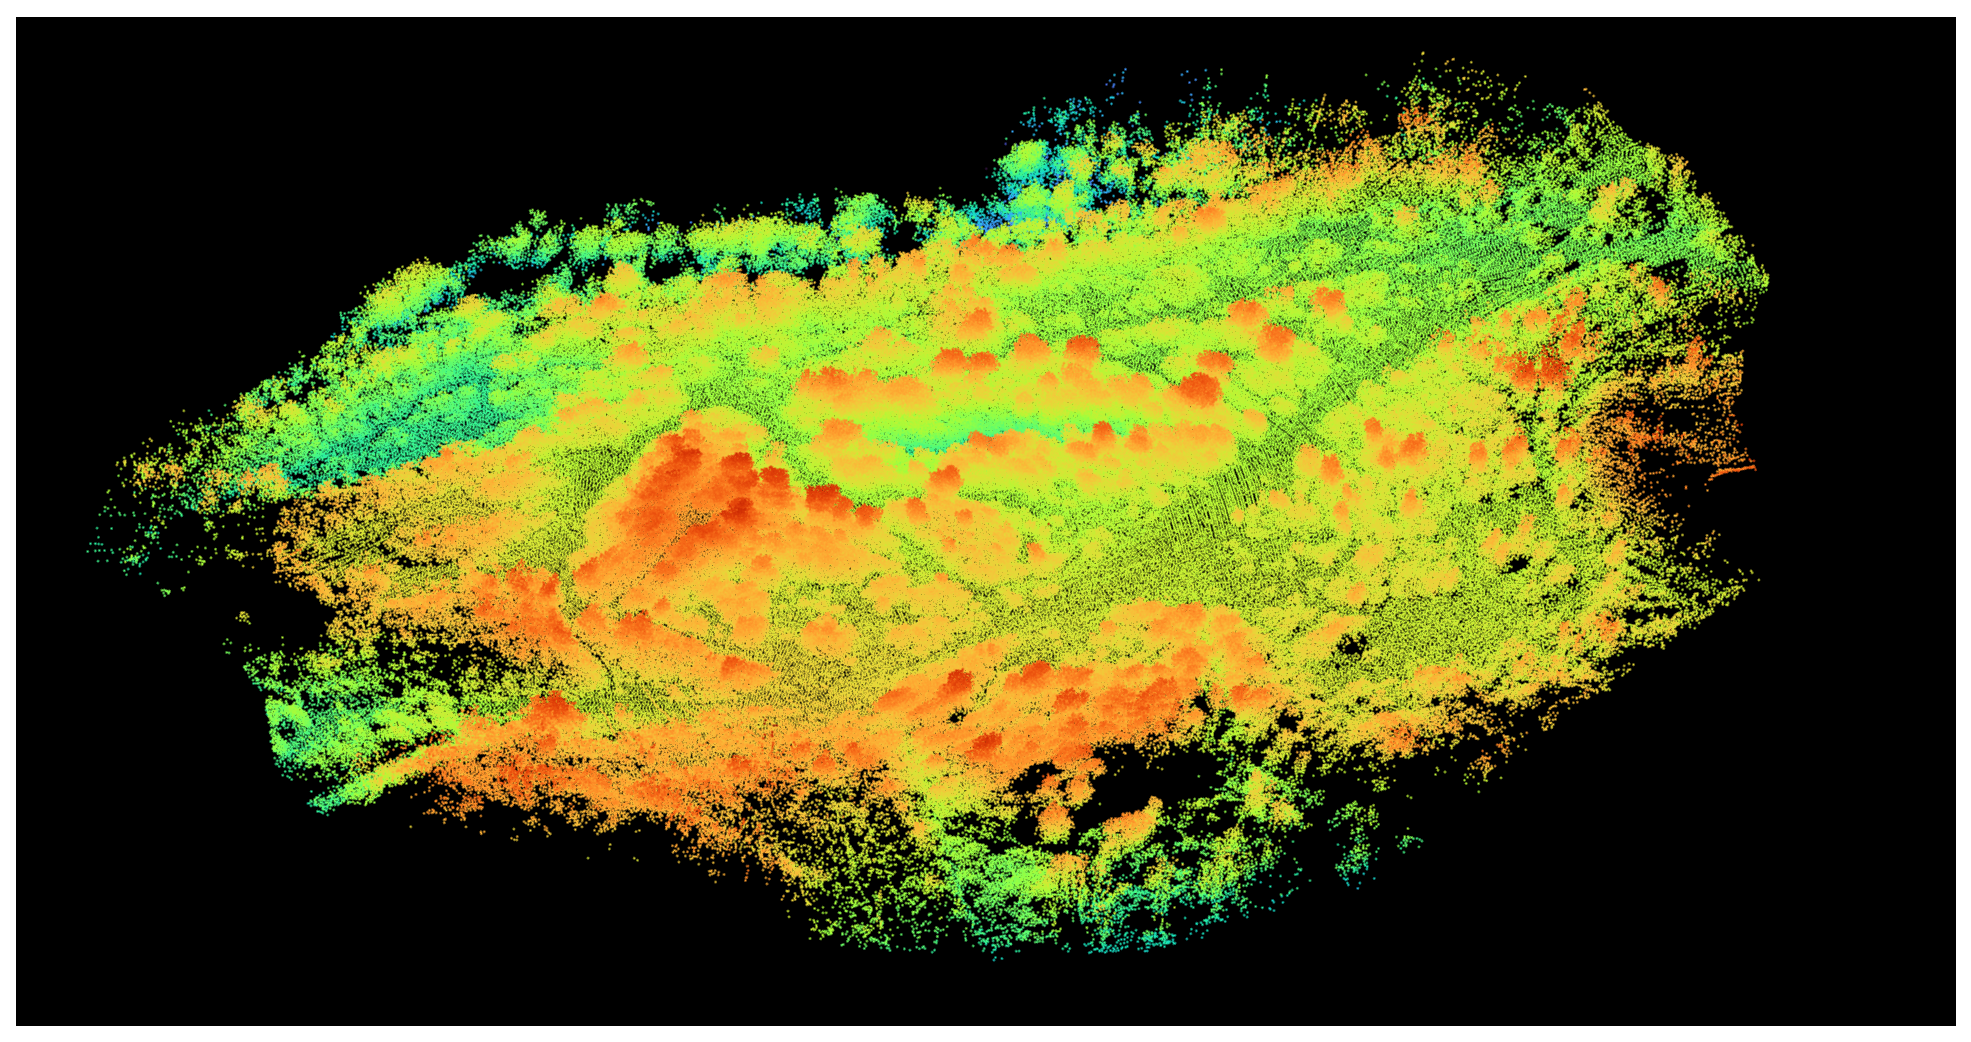
\includegraphics[width=0.5\textwidth]{figs/results/geometric_understanding/slam_ptCloud.eps}}\\%\\[20pt]   
   \subfloat[]{
        \label{fig:slam_hausdorff}         %% Etiqueta para la segunda subfigura
        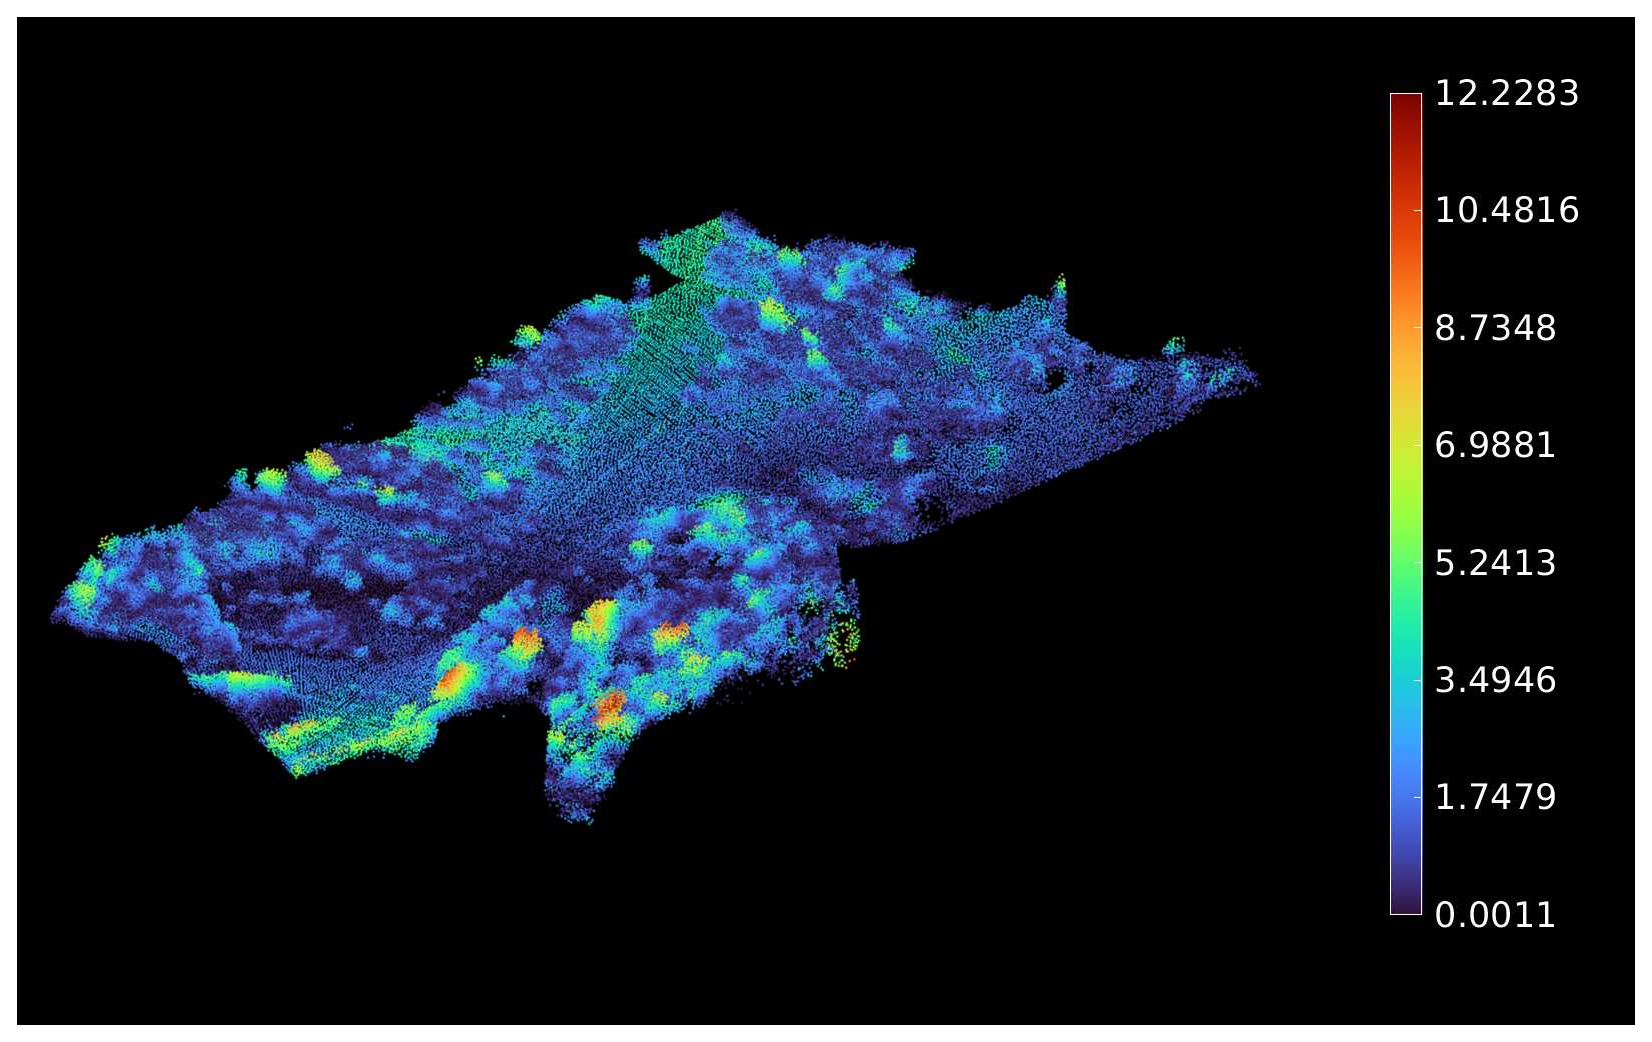
\includegraphics[width=0.5\textwidth]{figs/results/geometric_understanding/housedorff_distance.eps}}%\\[20pt]            
   \caption{Point cloud maps of the A) photogrammetry baseline, B) SLAM outcome. The two maps were compared using the Hausdorff distance, whose result is visualized as C) the SLAM map colored according to this metric. Note that the baseline and the SLAM clouds colormaps correspond to RGB and height values, respectively. Figure courtesy of Dr. Francisco Yandun.}
   \label{fig:results_mapping_slam}                %% Etiqueta para la figura entera
\end{figure*}

\begin{figure}
    \centering
    \includegraphics[width=\textwidth]{figs/results/3d_reconstruction.png}
    \caption{An example 3D reconstruction developed using Agisoft, a commercial structure from motion software.}
    \label{fig:3d_reconstrction}
\end{figure}


\section{Semantic mapping}

\begin{itemize}
    \item This is where we collected the data
    \item These are the sensors we used
    \item This is the flight pattern we flew
    \item What metrics do we use.
\end{itemize}
\subsection{Image segmentation}
\begin{figure}
    \centering
    \includegraphics[width=\textwidth]{figs/results/confusion_matrix.png}
    \caption{Confusion matrix semantics}
    \label{fig:res_confusion_matrix}
\end{figure}
\begin{figure*}[h!]
   \centering
   \includegraphics[width=0.5\textwidth]{figs/results/semantic_segmentation/Gascola/safeforest_all_classes_flat.png}
   \includegraphics[width=0.25\textwidth]{figs/results/semantic_segmentation/Gascola/safeforest_classmap_compressed_flat.png}
   
\includegraphics[width=0.80\textwidth]{figs/results/semantic_segmentation/Gascola/000000_rgb_img.png}
   \vspace{0pt}
   
\includegraphics[width=0.80\textwidth]{figs/results/semantic_segmentation/Gascola/000005_rgb_img.png}
   \vspace{0pt}
   
\includegraphics[width=0.80\textwidth]{figs/results/semantic_segmentation/Gascola/000010_rgb_img.png}
   \vspace{0pt}
   
\includegraphics[width=0.80\textwidth]{figs/results/semantic_segmentation/Gascola/000015_rgb_img.png}
   \vspace{0pt}
   \caption{
   Qualitative semantic mapping results from the test set. The results are shown both for the predicted classes and the aggregated ones, with colors visualized in the top rows.
   White regions in the ground truth represent areas that were ambiguous to the human annotator. Overall the predictions match the ground truth well and boundaries are well-defined. Note that many regions of confusions, such as canopy-to-trunk and green shrub to canopy, fall within the same coarse classes for our mapping purposes.
   }
   \label{fig:results_semantic_seg_qualitative}                %% Etiqueta para la figura entera
\end{figure*}



\section{Tree detection}

\begin{figure}[h]
    \subfloat{\includegraphics[width=0.45\textwidth]{figs/results/tree_detections/emerald_point_tree_detections.png}}
    \hfill
    \subfloat{\includegraphics[width=0.45\textwidth]{figs/results/tree_detections/stowe_anew_detections.png}}
    \caption{Visualizations of the proposed planning method on two different data images.}
    \label{fig:res_unpairqual}
\end{figure}

\section{Informative path planning}

\begin{figure}
    \centering
    \includegraphics[width=\textwidth]{figs/results/feature_extraction/Screenshot from 2023-05-19 10-03-18.png}
    \caption{Unsupervised features extracted from the data}
    \label{fig:res_unsupervised_feature_qual}
\end{figure}

\begin{figure}
    \centering
    \includegraphics[width=\textwidth]{example-image-a}
    \caption{Random satellite predictions using the features}
    \label{fig:sat_predictions}
\end{figure}


\begin{figure}[h]
    \subfloat{\includegraphics[width=0.45\textwidth]{figs/results/ipp/unpaired_qual_1 (1).png}}
    \hfill
    \subfloat{\includegraphics[width=0.45\textwidth]{figs/results/ipp/unpaired_qual_2 (1).png}}
    \caption{Visualizations of the proposed planning method on two different data images.}
    \label{fig:res_unpairqual}
\end{figure}


\begin{figure}[h]
    \subfloat{\includegraphics[width=0.45\textwidth]{figs/results/ipp/paired_qual_GBS-IPP (1).png}}
    \hfill
    \subfloat{\includegraphics[width=0.45\textwidth]{figs/results/ipp/paired_qual_pizza (1).png}}
    \caption{A comparison of the proposed method with a baseline}
    \label{fig:res_pairedqual}
\end{figure}

\begin{figure}[h]
    \subfloat{\includegraphics[width=0.3\textwidth]{figs/results/ipp/error (2).png}}
    \hfill
    \subfloat{\includegraphics[width=0.3\textwidth]{figs/results/ipp/balanced_error (2).png}}
    \hfill
    \subfloat{\includegraphics[width=0.3\textwidth]{figs/results/ipp/timing_result (1).png}}
    \caption{Quantitative statistics for IPP}
    \label{fig:res_ipp_quant}
\end{figure}

\subsection{Problem formulation}
The goal of the experiments is to model a realistic data collection scenario. The data is collected over a series of missions, where each mission must be fully planned before it is executed. Each mission is allowed a pathlength budget and a number of samples it is allowed to collection. 

In our experiments we use randomly-sampled NAIP tiles to evaluate the approach. In each situation the agent starts in the center of the environment and must return there after each mission.

In these experiments we use a very simple prediction system to predict the class of unobserved pixels. It is simply a nearest-neighbor classifier which operates on the same PCA-compressed MOSAIKS features that are used for planning. While simple, this approach is well-suited to the extremely low number of training samples used in this setting and the standardized and uncorrelated nature of our feature space.

Before any missions have been executed, the agent can only observe the label of the pixel it is at. Then it plans a mission and executes it, observing the labels at the chosen sampling locations. These samples are used to train a prediction model which is used for evaluation and, in theory, could be used to inform the plan for the next mission. 


The experiments were conducted over ten random domains, which each represented an 800x800px crop from the Chesapeake Bay land cover dataset. Each tile represents approximately half a kilometer square. The pathlength was set as 800 pixels as well, which meant that the agent could go to one side of the environment and return to the start within the budget but some corners were completely unreachable. Each domain was explored using four missions where 10 samples could be collected during each one. Each sample meant the agent could observe the class of one pixel. After each mission, the class of all pixels  were predicted using the nearest neighbor classifier and the error metrics were computed. 


\begin{itemize}
    \item In some settings the remote sensing data was just downsampled from the highest resulotion 
\end{itemize}

\subsection{Baselines}
\begin{itemize}
    \item Geometrics planners, e.g. pizza or coverage 
    \item Ergodic planner \cite{Rao}
    \item Greedy baselines?
\end{itemize}

\subsection{Metrics}
The quality of the predictions are evaluated on two metrics, accuracy and averaged recall. The first is simply the fraction of pixels in the map that were assigned the correct class label by the prediction system. The second represents the average of the per class recalls. This metric is chosen so that rare classes are treated equally in the evaluation procedure, since this is critically important when we explicitly want to find rare classes. We also report the time taken to generate the plan. Note that this does not include the time taken to generate the class predictions, since the planner is agnostic to the choice of prediction algorithm.



